%ankicard
%ankitags mathematics algebra precalculus
\subsection{What are the notations of intervals?}
%ankifront

\begin{small}
    \begin{tabularx}{1\textwidth}{
        p{\dimexpr1\textwidth\relax}
    }
    \toprule
    \textbf{What are the notations of intervals?} \\
    \bottomrule
    \end{tabularx}
\end{small}
%ankifront end
%ankiback

\begin{small}
\begin{tabularx}{1\textwidth}{
    p{\dimexpr0.3\textwidth\relax}
    p{\dimexpr0.3\textwidth\relax}
    p{\dimexpr0.4\textwidth\relax}
}
\toprule
Notation & Set Description & Graph \\
\midrule

$ \left( a,b \right) $ &
$ \left\{ x | a < x < b \right\} $ &
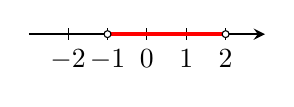
\begin{tikzpicture}[scale=0.5]
  % Drawing the real number line
  \draw[thick, -stealth] (-3,0) -- (3,0); % Main line with arrow
  \foreach \x in {-2,-1,0,1,2} {
    \draw (\x,0.15) -- (\x,-0.15) node[below] {$\x$}; % Tick marks and labels
  }
  % \draw (0,0.3) -- (0,-0.3) node[below] {$0$}; % Emphasize origin

  % Marking the interval [-2, 3)
  \draw[line width=1.5pt, red] (-1,0) -- (2,0); % Thick line for interval
  \draw[black, fill=white] (-1,0) circle (2.5pt); % Closed endpoint at -2
  \draw[black, fill=white] (2,0) circle (2.5pt); % Open endpoint at 3
\end{tikzpicture}
\\
\midrule

$ \lbrack a,b \rbrack $ &
$ \left\{ x | a \leq x \leq b \right\} $ &
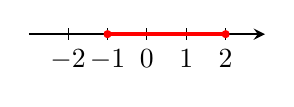
\begin{tikzpicture}[scale=0.5]
  % Drawing the real number line
  \draw[thick, -stealth] (-3,0) -- (3,0); % Main line with arrow
  \foreach \x in {-2,-1,0,1,2} {
    \draw (\x,0.15) -- (\x,-0.15) node[below] {$\x$}; % Tick marks and labels
  }
  % \draw (0,0.3) -- (0,-0.3) node[below] {$0$}; % Emphasize origin

  % Marking the interval [-2, 3)
  \draw[line width=1.5pt, red] (-1,0) -- (2,0); % Thick line for interval
  \filldraw[red] (-1,0) circle (2.5pt); % Closed endpoint at -2
  \filldraw[red] (2,0) circle (2.5pt); % Open endpoint at 3
\end{tikzpicture}
\\
\midrule

$ \lbrack a,b ) $ &
$ \left\{ x | a \leq x < b \right\} $ &
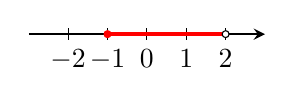
\begin{tikzpicture}[scale=0.5]
  % Drawing the real number line
  \draw[thick, -stealth] (-3,0) -- (3,0); % Main line with arrow
  \foreach \x in {-2,-1,0,1,2} {
    \draw (\x,0.15) -- (\x,-0.15) node[below] {$\x$}; % Tick marks and labels
  }
  % \draw (0,0.3) -- (0,-0.3) node[below] {$0$}; % Emphasize origin

  % Marking the interval [-2, 3)
  \draw[line width=1.5pt, red] (-1,0) -- (2,0); % Thick line for interval
  \filldraw[red] (-1,0) circle (2.5pt); % Closed endpoint at -2
  \draw[black, fill=white] (2,0) circle (2.5pt); % Open endpoint at 3
\end{tikzpicture}
\\

\midrule
$ ( a,b \rbrack $ &
$ \left\{ x | a < x \leq b \right\} $ &
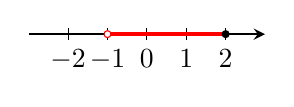
\begin{tikzpicture}[scale=0.5]
  % Drawing the real number line
  \draw[thick, -stealth] (-3,0) -- (3,0); % Main line with arrow
  \foreach \x in {-2,-1,0,1,2} {
    \draw (\x,0.15) -- (\x,-0.15) node[below] {$\x$}; % Tick marks and labels
  }
  % \draw (0,0.3) -- (0,-0.3) node[below] {$0$}; % Emphasize origin

  % Marking the interval [-2, 3)
  \draw[line width=1.5pt, red] (-1,0) -- (2,0); % Thick line for interval
  \draw[red, fill=white] (-1,0) circle (2.5pt); % Closed endpoint at -2
  \filldraw[black] (2,0) circle (2.5pt); % Open endpoint at 3
\end{tikzpicture}
\\
\midrule

$ ( a,\infty ) $ &
$ \left\{ x | a < \infty \right\} $ &
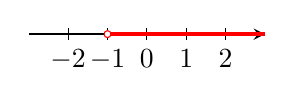
\begin{tikzpicture}[scale=0.5]
  % Drawing the real number line
  \draw[thick, -stealth] (-3,0) -- (3,0); % Main line with arrow
  \foreach \x in {-2,-1,0,1,2} {
    \draw (\x,0.15) -- (\x,-0.15) node[below] {$\x$}; % Tick marks and labels
  }
  % \draw (0,0.3) -- (0,-0.3) node[below] {$0$}; % Emphasize origin

  % Marking the interval [-2, 3)
  \draw[line width=1.5pt, red] (-1,0) -- (3,0); % Thick line for interval
  \draw[red, fill=white] (-1,0) circle (2.5pt); % Closed endpoint at -2
  % \filldraw[black] (2,0) circle (2.5pt); % Open endpoint at 3
\end{tikzpicture}
\\
\midrule

$ \lbrack a,\infty ) $ &
$ \left\{ x | a \leq \infty \right\} $ &
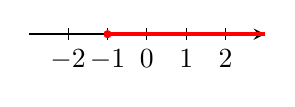
\begin{tikzpicture}[scale=0.5]
  % Drawing the real number line
  \draw[thick, -stealth] (-3,0) -- (3,0); % Main line with arrow
  \foreach \x in {-2,-1,0,1,2} {
    \draw (\x,0.15) -- (\x,-0.15) node[below] {$\x$}; % Tick marks and labels
  }
  % \draw (0,0.3) -- (0,-0.3) node[below] {$0$}; % Emphasize origin

  % Marking the interval [-2, 3)
  \draw[line width=1.5pt, red] (-1,0) -- (3,0); % Thick line for interval
  \filldraw[red] (-1,0) circle (2.5pt); % Closed endpoint at -2
  % \filldraw[black] (2,0) circle (2.5pt); % Open endpoint at 3
\end{tikzpicture}
\\
\midrule

$ ( -\infty, a ) $ &
$ \left\{ x | x < a \right\} $ &
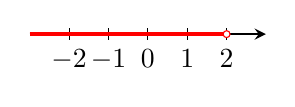
\begin{tikzpicture}[scale=0.5]
  % Drawing the real number line
  \draw[thick, -stealth] (-3,0) -- (3,0); % Main line with arrow
  \foreach \x in {-2,-1,0,1,2} {
    \draw (\x,0.15) -- (\x,-0.15) node[below] {$\x$}; % Tick marks and labels
  }
  % \draw (0,0.3) -- (0,-0.3) node[below] {$0$}; % Emphasize origin

  % Marking the interval [-2, 3)
  \draw[line width=1.5pt, red] (-3,0) -- (2,0); % Thick line for interval
  \draw[red, fill=white] (2,0) circle (2.5pt); % Closed endpoint at -2
  % \filldraw[black] (2,0) circle (2.5pt); % Open endpoint at 3
\end{tikzpicture}
\\
\midrule

$ ( -\infty, a \rbrack $ &
$ \left\{ x | x \leq a \right\} $ &
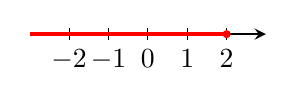
\begin{tikzpicture}[scale=0.5]
  % Drawing the real number line
  \draw[thick, -stealth] (-3,0) -- (3,0); % Main line with arrow
  \foreach \x in {-2,-1,0,1,2} {
    \draw (\x,0.15) -- (\x,-0.15) node[below] {$\x$}; % Tick marks and labels
  }
  % \draw (0,0.3) -- (0,-0.3) node[below] {$0$}; % Emphasize origin

  % Marking the interval [-2, 3)
  \draw[line width=1.5pt, red] (-3,0) -- (2,0); % Thick line for interval
  \filldraw[red] (2,0) circle (2.5pt); % Closed endpoint at -2
  % \filldraw[black] (2,0) circle (2.5pt); % Open endpoint at 3
\end{tikzpicture}
\\
\midrule

$ ( -\infty, \infty ) $ &
$ \mathbb{R} \text{set of real numbers} $ &
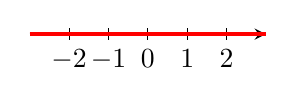
\begin{tikzpicture}[scale=0.5]
  % Drawing the real number line
  \draw[thick, -stealth] (-3,0) -- (3,0); % Main line with arrow
  \foreach \x in {-2,-1,0,1,2} {
    \draw (\x,0.15) -- (\x,-0.15) node[below] {$\x$}; % Tick marks and labels
  }
  % \draw (0,0.3) -- (0,-0.3) node[below] {$0$}; % Emphasize origin

  % Marking the interval [-2, 3)
  \draw[line width=1.5pt, red] (-3,0) -- (3,0); % Thick line for interval
  % \filldraw[red] (2,0) circle (2.5pt); % Closed endpoint at -2
  % \filldraw[black] (2,0) circle (2.5pt); % Open endpoint at 3
\end{tikzpicture}
\\
\midrule

\end{tabularx}
\end{small}
%ankiback end
